\documentclass[aspectratio=169]{beamer}
\usepackage{graphicx}
\title{Using agent-based modelling to explore the effect of social networks and beliefs on active travel}
\author{Robert Greener}
\institute{London School of Hygiene and Tropical Medicine}
\date{27th October 2022}

\begin{document}
\maketitle

\begin{frame}
    \frametitle{Background}
    \begin{columns}
        \begin{column}{0.5\textwidth}
            \begin{itemize}
                \item Active travel policies frame walking \& cycling as `good', cars as `bad'!
                \item Perceptions of acceptable commute method vary by groups.
                \item Beliefs may explain this difference.
                \item Beliefs spread through social networks.
            \end{itemize}
        \end{column}
        \begin{column}{0.5\textwidth}
            \begin{figure}[H]
                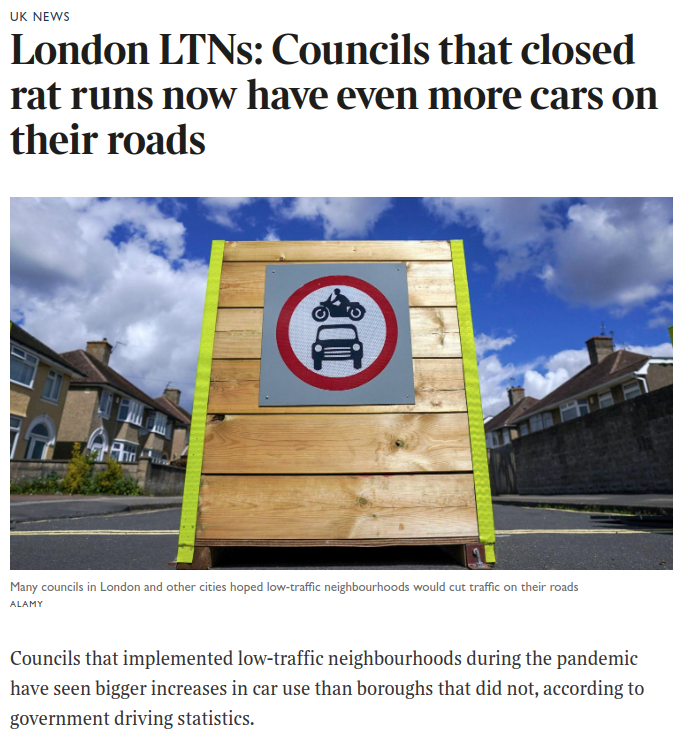
\includegraphics[width=0.7\textwidth]{figures/the-times.png}
                \caption{\emph{The Times} 24th October 2022}
            \end{figure}
        \end{column}
    \end{columns}
\end{frame}

\begin{frame}
    \frametitle{Research questions}
    \begin{enumerate}
        \item What are the beliefs and attitudes required to create a calibrated model of active travel?
              \begin{itemize}
                  \item Answered by a systematic review of the literature.
              \end{itemize}
        \item What network-based interventions may be effective in increasing active travel levels?
        \item How may non-network-based interventions cause an additional network-based effect
    \end{enumerate}
\end{frame}

\begin{frame}
    \frametitle{Elements of the model}
    \begin{itemize}
        \item \emph{Beliefs}: These are `attitudes towards some proposition'.
        \item \emph{Behaviours}: These are actions an agent can perform.
        \item \emph{Agents}: These are people (in this model).
    \end{itemize}
\end{frame}

\begin{frame}
    \frametitle{Agents hold beliefs}
    \begin{itemize}
        \item Agents hold beliefs either positively or negatively (i.e., they are averse to the belief).
        \item For example, John may believe that cycling to work makes you look cool; Alex might be averse to that view.
        \item This strength of feeling is called \emph{activation}.
        \item It is a numerical value in the range \([-1,+1]\).
        \item This determines the behaviour agents perform; however, this is out-of-scope for this model as there already exist good models for this (\emph{BDI}).
    \end{itemize}
\end{frame}

\begin{frame}
    \frametitle{Beliefs interact}
    \begin{itemize}
        \item Beliefs interact with one another.
        \item Holding one belief may make it more likely that you hold another, less likely, or have no effect.
        \item For example, consider belief \emph{A}: Cycling is good for the environment and belief \emph{B}: Climate change is exaggerated.
        \item If you hold \emph{B}, you will be less likely to hold \emph{A}.
        \item This relationship is defined as a numerical value in the range \([-1, +1]\).
    \end{itemize}
\end{frame}

\begin{frame}
    \frametitle{Behaviours are how we perceive the beliefs of others}
    \begin{itemize}
        \item We cannot know what others believe directly; we \emph{perceive} this through their actions.
        \item We can observe what others are likely to believe based upon what they do.
        \item This is a numerical value between \([-1, +1]\).
        \item For example, consider someone cycles.
        \item They are possibly driven by the belief that cycling is good for the environment.
        \item They are unlikely to believe the climate change is exaggerated.
    \end{itemize}
\end{frame}

\begin{frame}
    \frametitle{Putting this all together}
    \begin{itemize}
        \item Agents belong to a social network, represented as a weighted digraph.
        \item Each day agents observe what their friends perform.
        \item They then use this to determine what they believe (\emph{perceiving}).
        \item Taking into account how close their friends are, and the beliefs they already hold, they update their beliefs (to conform).
        \item They then perform actions of their own based upon their beliefs (through BDI).
    \end{itemize}
\end{frame}

\begin{frame}
    \frametitle{How do we find the real beliefs?}
    \begin{itemize}
        \item The challenge with using this model is to find real beliefs about active travel.
        \item i.e., parameterisation.
        \item To parameterise it, I'm conducting a systematic review of the literature.
        \item This is a process where a structured search query is used to search databases.
        \item This returned about 15,000 hits. Of this about 200 studies are included.
        \item The beliefs, and their effect on behaviour, are extracted from these studies.
        \item The studies are also quality assessed.
        \item The results of this are plugged into this model.
    \end{itemize}
\end{frame}

\begin{frame}
    \frametitle{Next steps}
    \begin{itemize}
        \item Run this model many times. Do the results make sense?
        \item Implement some interventions. What are there results?
        \item What do the results mean for public health policy / planning policy?
        \item Is there any `low-hanging fruit'?
    \end{itemize}
\end{frame}

\begin{frame}
    \frametitle{Any questions / acknowledgements}
    \begin{itemize}
        \item Thank you for listening; any questions?
        \item Robert Greener is supported by a Medical Research Council Studentship [grant number: MR/N0136638/1].
    \end{itemize}
    \vspace*{4em}
    
\includegraphics[height=5em]{figures/LSHTM-logo-bw.jpg}
    
\includegraphics[height=5em]{figures/Medical_Research_Council_logo.svg.png}
    
\includegraphics[height=2em]{figures/philab.png}
\end{frame}
\end{document}